\part{CODEC}

Para realizar aplicaciones con audio en la placa XSB Board \cite{XSBBoard} de que se dispone en el laboratorio de la asignatura, el primer paso a dar es realizar un driver en hardware para el codec\footnote{En este caso un codec se refiere a un conversor analógico-digital y otro digital-analógico, ambos estéreo, y no de un codificador-descodificador en el sentido de conversión entre formatos. A lo largo de la memoria en ocasiones se nombrará a los conversores como ADC y DAC respectivamente.} de audio que incluye dicha placa, concretamente el ASAHI KASEI AK4565 \cite{AK4565}.

	
	
\section{Desarrollo seguido}

	\subsection{Estudio de datasheets}
		El primer paso del desarrollo fue el estudio de los datasheets, tanto del codec como el de la placa. Del documento de la placa se obtuvo principalmente qué pines de la FPGA se conectaban con el codec en qué manera, lo cual puede verse resumido en la siguiente tabla:


\begin{figure}[H]

\centering
	\begin{tabular}{|c|c|c|c|c|}
		\hline
		\textbf{FPGA pin} & \textbf{Net name} & \textbf{Codec pin} & \textbf{Prog. Osc. pin}\\
		\hline
		141 (D2) & PB-D2 & CDTO &\\
		\hline
		145 (D1) & PB-D1 & CDTI &\\
		\hline
		153 (DIN/D0) & PB-D0 & CCLK &\\
		\hline
		165 & AU-CSN\# & CSN\# &\\
		\hline
		166 &  AU-BCLK & BCLK &\\
		\hline
		167 &  AU-MCLK & MCLK &\\
		\hline
		168 &  AU-LRCK & LRCK &\\
		\hline
		169 &  AU-SDTI & SDTI &\\
		\hline
		173 &  AU-SDTO0 & SDTO0 &\\
		\hline
		77 (I/GCK1) & FPGA-CLK1 & & CLKD\\
		\hline
	\end{tabular}

  \caption{Relación de conexiones entre FPGA, codec y oscilador programable.}
\end{figure}


Del datasheet del codec... Palabras de configuración a cambiar: entradas, loopback, selección de interfaz de audio.


	\subsection{Relojes}

		Modulo IS2\_CLOCKS.vhd (revisar)
	

	\subsection{Loopback analógico}

		Configurando el codec para que tomase como entrada la conexión LINE IN y activando el loopback analógico incluido en el codec, comprobamos que el modulo que envía la configuración al codec funcionaba correctamente, puesto que ninguna de las dos opciones estaba configurada por defecto y tras arrancar la FPGA y mandar esta configuración, el audio que entraba por LINE IN llegaba a la salida.
		
	
	\subsection{Interfaz I$^2$S}

		El codec de audio permite utilizar varios interfaces de audio. De ellos elegimos I$^2$S por ser un estándar. Entonces, realizamos un módulo que se comúnicase con el codec utilizando este estándar para enviar y recibir información de audio (I2S.vhd). A partir de ahora, en vez de enviar la configuración de activación del loopback, enviamos la selección de I$^2$S como interfaz de audio.

	\subsection{Loopback digital}
		
		Para probar el módulo I2S que se encarga de la interfaz de audio, realizamos un modulo extremadamente sencillo consistente en unir las salidas del conversor digital-analógico con las entradas del conversor analógico digital de dicho módulo. El resultado es el mismo que el obtenido con el loopback analógico, pero ahora el audio está siendo convertido a digital en el codec, llevado a la FPGA, devuelto al codec y convertido de nuevo a analógico.

		

	
\section{Problemas encontrados}

	

	\subsection{Canales cruzados}

		Quisimos comprobar que cada canal de audio (izquierdo y derecho) estaba siendo tratado como tal y no se estaban intercambiando. Para ello hicimos uso de archivos de audio lanzados desde el ordenador, de los cuales eramos capaces de distinguir con facilidad el canal izquierdo del derecho. Las pruebas que realizamos son las siguientes:

		\paragraph{Conexion sin cruzar canales}
			En esta prueba conectamos el canal izquierdo del ADC con el canal izquierdo del DAC, haciendo lo mismo con el canal derecho. Los canales se reproducían correctamente, cada uno en su respectivo lado.


		\paragraph{Conexion cruzando canales}
			En esta prueba conectamos el canal izquierdo del ADC con el canal derecho del DAC y el canal derecho del ADC con el canal izquiero del DAC. Los canales se reproducían cruzados, es decir, por el canal izquierdo se escuchaba el derecho y viceversa, como era de esperar. En este momento llegamos a la conclusión, que más tarde se verá errónea, de que los canales eran tratados de forma correcta. Una imagen que ilustra lo que sucede en la placa es la siguiente:
\begin{figure}[h]
\begin{center}
	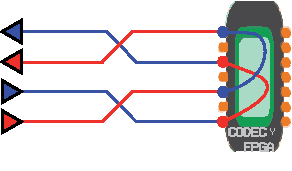
\includegraphics[width=0.5\textwidth]{./swapping_channels-eps-converted-to}
\caption{Cruce tanto a la entrada como a la salida de los conectores jack}
\end{center}
\end{figure}

		\paragraph{Utilización de un sólo canal de entrada y procesado diferente en cada canal de salida}
	
			Más tarde, ya trabajando con una aplicación que hacía uso del codec de audio...
			
		
	
\section{Documentación para la reutilización del codec}
	
